\documentclass[10pt]{beamer}

%%%
% PREAMBLE FOR THIS DOC 
%%%
%https://tex.stackexchange.com/questions/68821/is-it-possible-to-create-a-latex-preamble-header
\usepackage{/Users/miw267/Repos/latex_preamble/beamer_preamble}


%%%
% PREAMBLE SPECIAL FOR THIS DECK
%%%
\definecolor{condred}{RGB}{200,30,30}
\definecolor{accessgreen}{RGB}{30,160,60}
\usetikzlibrary{calc}


%%% TRY TO RESHOW TOC AT EACH SECTION START (with current section highlighted)
% Reference: https://tex.stackexchange.com/questions/280436/how-to-highlight-a-specific-section-in-beamer-toc
\newcommand\tocforsect[2]{%
  \begingroup
  \edef\safesection{\thesection}
  \setcounter{section}{#1}
  \tableofcontents[#2,currentsection]
  \setcounter{section}{\safesection}
  \endgroup
}



%%%
% DOCUMENT
%%%

\begin{document}

%\maketitle

%% Title page frame
%\begin{frame}
%    \titlepage 
%\end{frame}





\title{10/19/2026: Multiple Proofs}
\author{CSCI 246: Discrete Structures}
\date{Textbook reference: Ch. 2, Hampkins}

\begin{frame}
    \titlepage 
\end{frame}


\begin{frame}


%\begin{mygreenbox}[title=Quiz Set up]
%\begin{itemize}
%\item \textbf{Guest lecturer Monday}: Paul Cornish.   
%\end{itemize}
%\end{mygreenbox}
%
%\vfill 

\begin{myyellowbox}[title=Today's Agenda]
\begin{itemize}
	\item Proof Jigsaw
	\item (If time) Review previous group exercises
\end{itemize}

\end{myyellowbox}

\end{frame}

\begin{frame}{Why multiple proofs?}

Once you've proved a theorem, you know it's true.  So why would you ever want a second proof?

\vfill
\pause
\begin{enumerate}
\item \textbf{Confidence.} Two independent arguments make an error less likely (like testing code against a second implementation). \pause
\item \textbf{Understanding.} Different proofs explain \textit{why} the theorem is true from different angles (cases, algebra, pictures, counting, \ldots). \pause
\item \textbf{Generalization.} Different proofs suggest different generalizations.  (Hamkins' main point.)
\end{enumerate}
\end{frame}



\begin{frame}[plain]
\begin{tikzpicture}[remember picture, overlay]
  % Background image, stretched to fill the whole slide
  \node[inner sep=0pt] at (current page.center)
    {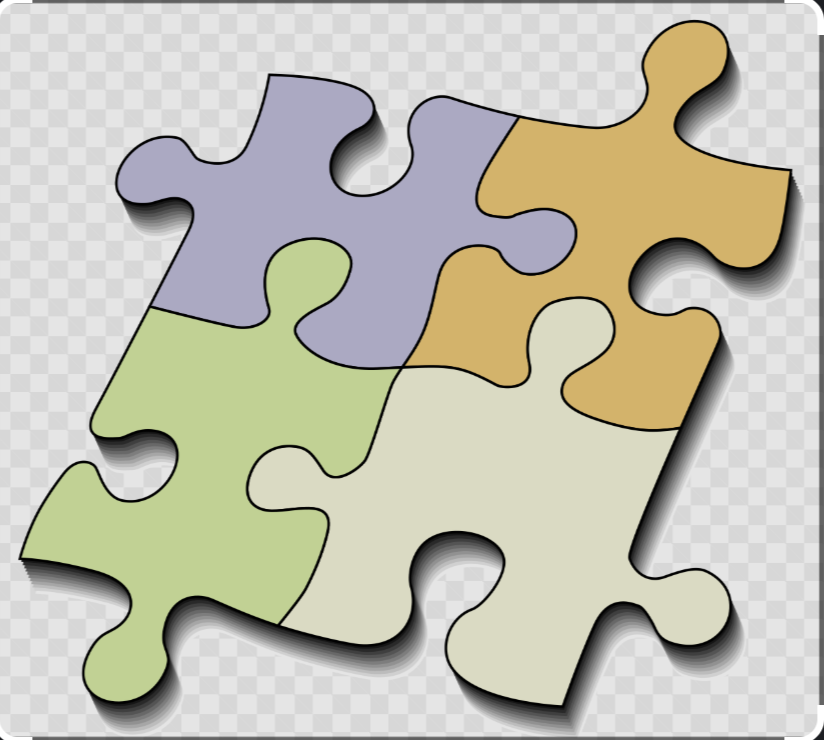
\includegraphics[width=\paperwidth, height=\paperheight]{images/jigsaw}};
  % Optional dark tint so the text stays readable on any photo
  \fill[black, opacity=0.35] (current page.south west) rectangle (current page.north east);
  % Large centered text
  \node[text=white, font=\Huge\bfseries, align=center, text width=0.85\paperwidth]
    at (current page.center) {Proof Jigsaw};
\end{tikzpicture}
\end{frame}


\begin{frame}
\footnotesize 
\begin{mybluebox}[title=Theorem]
For any natural number $n$, the number $n^2-n$ is even.	
\end{mybluebox}

\begin{itemize}
\item \textbf{Proof \#1: By Cases.}  Miller, Maverick; Moss, Emily; Neuman, Evan; Thompson, Jaiden; Vath, Ethan \\
\item \textbf{Proof \#2: By High-School Algebra.} Lee, Holden; Fellows, Audrey; Horner, Jayden; Mousseau, Matthew; Roberts, Matthew \\
\item \textbf{Proof \#3: By Induction.} Blaisdell, Olyver; Fuller, Ryan; Hager, Nathan; Kintzel, Samantha; Mcbride, Daniel \\
\item \textbf{Proof \#4: By Geometrical Figure.} Ashley, Isabelle; Bailey, Tanna; Cardenas, Dominic; Fabik, Roland; Shevtsov, Timothy \\
\item \textbf{Proof \#5: By Combinatorics.} Griffen, Clara; Grutsch, Tanner; Mayala, Reece; Ramos, Vydel; Roller, Nathan \\
\item \textbf{Proof \#6: By Modular Arithmetic.} Cutler, George; Fitzgerald, Ryan; McLean, Connor; Putnam, John; Thiessen, Logan \\
\item \textbf{Proof \#7: By Summation Identity.}  Johnson, Jaret; Lameres, Alexis; Rathbun, Jedidiah; Ryan, Otis; Stensland, Emma \\
\end{itemize}

\begin{mygreenbox}[title=Extensibility]
Which of your proofs still works if we replace 2 with 3? With 4?	
\end{mygreenbox}

\end{frame}

\end{document}


\begin{frame}{Group exercises}

\begin{enumerate}
\item (Hamkins Ex. 2.1, first part) Prove that the sum, difference, and product of two even numbers is even.
\item (Hamkins Ex. 2.1, second part) Prove that the sum and difference of two odd numbers is even, but the product of two odd numbers is odd.
\end{enumerate}
\end{frame}



%
\begin{frame}{Solution to group exercise \#1}

\footnotesize 

\textbf{Proposition.} The sum, difference, and product of two even numbers is even.
\vfill 
\textbf{Proof.}
\begin{tabularx}{\textwidth}{|L{3.5cm}|X|}
\hline \textbf{Annotation} & \textbf{Main Text} \\ \hline
 \hlorange{Convert Prop. to ``if-then" form} &  \hlorange{We show that if $x$ and $y$ are even integers, then $x+y$, $x-y$, and $xy$ are even.} \\ \hline
\hlblue{State assumption (\qq{if})} & \hlblue{Let $x$ and $y$ be even integers} \\ \hline
\hlgreen{Unravel defs.} & \hlgreen{What goes here!?} \\ \hline
\hlred{*** The glue ***} &  \\
\hline
\hlgreen{Unravel defs.} & \hlgreen{What goes here!?} \\ 
\hline
  \hlblue{State conclusion (\qq{then})} & \hlblue{Hence, $x+y, x-y$ and $xy$ are even.} \\ \hline
\hline
\end{tabularx}
\end{frame}
%
%

%
\begin{frame}{Solution to group exercise \#1}

\footnotesize 

\textbf{Proposition.} The sum, difference, and product of two even numbers is even.
\vfill 
\textbf{Proof.}
\begin{tabularx}{\textwidth}{|L{3.5cm}|X|}
\hline \textbf{Annotation} & \textbf{Main Text} \\ \hline
 \hlorange{Convert Prop. to ``if-then" form} &  \hlorange{We show that if $x$ and $y$ are even integers, then $x+y$, $x-y$, and $xy$ are even.} \\ \hline
\hlblue{State assumption (\qq{if})} & \hlblue{Let $x$ and $y$ be even integers} \\ \hline
\hlgreen{Unravel defs.} & \hlgreen{Then by the definition of even, there exist integers $a,b$ such that $x=2a$ and $y=2b$.} \\ \hline
\hlred{*** The glue ***} & \hlred{What goes here?!?!} \\
\hline
 \hlgreen{Unravel defs.} & \hlgreen{So there are integers $c,d,e$ such that $x+y=2c$, $x-y=2d$, and $xy=2e$.} \\ \hline
  \hlblue{State conclusion (\qq{then})} & \hlblue{Hence, $x+y, x-y$ and $xy$ are even.} \\ \hline
\hline
\end{tabularx}
\end{frame}
%
%

\begin{frame}{Solution to group exercise \#1}
\footnotesize 
\textbf{Proposition.} The sum, difference, and product of two even numbers is even.
\vfill 
\textbf{Proof.}

\begin{tabularx}{\textwidth}{|L{3.5cm}|X|}
\hline \textbf{Annotation} & \textbf{Main Text} \\ \hline
\hlorange{Convert Prop. to \qq{if-then} form} &  \hlorange{We show that if $x$ and $y$ are even integers, then $x+y$, $x-y$, and $xy$ are even.} \\ \hline
\hlblue{State assumption (\qq{if})} & \hlblue{Let $x$ and $y$ be even integers} \\ \hline
\hlgreen{Unravel defs.} & \hlgreen{Then by the definition of even, there exist integers $a,b$ such that $x=2a$ and $y=2b$.} \\ \hline
\hlred{*** The glue ***} & 
\hlred{We have:
\[
\begin{aligned}
x+y &= 2a + 2b = 2\explaintermbrace{$\defeq c$}{(a+b)} \\	
x-y &= 2a - 2b = 2\explaintermbrace{$\defeq d$}{(a-b)} \\
xy  &= 2a \cdot 2b = 2\explaintermbrace{$\defeq e$}{(2ab)}  
\end{aligned}
\]
}
\\ \hline
 \hlgreen{Unravel defs.} & \hlgreen{So there are integers $c,d,e$ such that $x+y=2c$, $x-y=2d$, and $xy=2e$.} \\ \hline
  \hlblue{State conclusion (\qq{then})} & \hlblue{Hence, $x+y, x-y$ and $xy$ are even.} \\ \hline
\hline
\end{tabularx}
\end{frame}


\begin{frame}{Solution to group exercise \#2}
\footnotesize 
\textbf{Proposition.} The sum and difference of two odd numbers is even, but the product of odd numbers is odd.
\vfill 
\textbf{Proof.}

\begin{tabularx}{\textwidth}{|L{3.5cm}|X|}
\hline \textbf{Annotation} & \textbf{Main Text} \\ \hline
 \hlorange{Convert Prop. to ``if-then"} &  \hlorange{We show that if $x$ and $y$ are odd integers, then $x+y$ and $x-y$ are even, but $xy$ is odd.} \\ \hline
\hlblue{State ``if"} & \hlblue{Let $x$ and $y$ be odd integers.} \\ \hline
\hlgreen{Unravel defs.} & \hlgreen{What goes here?!?!} \\ \hline
\hlred{*** The glue ***} &  \\ \hline
\\ \hline
 \hlgreen{Unravel defs.} & \hlgreen{What goes here?!?!} \\ \hline
  \hlblue{State ``then"} & \hlblue{Hence,  $x+y$ and $x-y$ are even, but $xy$ is odd.} \\ \hline
\hline
\end{tabularx}
\end{frame}



\begin{frame}{Solution to group exercise \#2}
\footnotesize 
\textbf{Proposition.} The sum and difference of two odd numbers is even, but the product of odd numbers is odd.
\vfill 
\textbf{Proof.}

\begin{tabularx}{\textwidth}{|L{3.5cm}|X|}
\hline \textbf{Annotation} & \textbf{Main Text} \\ \hline
 \hlorange{Convert Prop. to ``if-then"} &  \hlorange{We show that if $x$ and $y$ are odd integers, then $x+y$ and $x-y$ are even, but $xy$ is odd.} \\ \hline
\hlblue{State ``if"} & \hlblue{Let $x$ and $y$ be odd integers.} \\ \hline
\hlgreen{Unravel defs.} & \hlgreen{Then by the definition of odd, there exist integers $a,b$ such that $x=2a+1$ and $y=2b+1$.} \\ \hline
\hlred{*** The glue ***} & \hlred{What goes here?!?!} \\ \hline
\\ \hline
 \hlgreen{Unravel defs.} & \hlgreen{So there are integers $c,d,e$ such that $x+y=2c$, $x-y=2d$, and $xy=2e+1$.} \\ \hline
  \hlblue{State ``then"} & \hlblue{Hence,  $x+y$ and $x-y$ are even, but $xy$ is odd.} \\ \hline
\hline
\end{tabularx}
\end{frame}




\begin{frame}{Solution to group exercise \#2}
\footnotesize 
\textbf{Proposition.} The sum and difference of two odd numbers is even, but the product of odd numbers is odd.
\vfill 
\textbf{Proof.}

\begin{tabularx}{\textwidth}{|L{2cm}|X|}
\hline \textbf{Annotation} & \textbf{Main Text} \\ \hline
 \hlorange{Convert Prop. to ``if-then"} &  \hlorange{We show that if $x$ and $y$ are odd integers, then $x+y$ and $x-y$ are even, but $xy$ is odd.} \\ \hline
\hlblue{State ``if"} & \hlblue{Let $x$ and $y$ be odd integers.} \\ \hline
\hlgreen{Unravel defs.} & \hlgreen{Then by the definition of odd, there exist integers $a,b$ such that $x=2a+1$ and $y=2b+1$.} \\ \hline
\hlred{* The glue *} & 
\scriptsize
\hlred{We have:
\[
\begin{aligned}
x+y &= (2a+1) + (2b+1) = 2a+2b+2 = 2\explaintermbrace{$\defeq c$}{(a+b+1)} \\	
x-y &= (2a+1) - (2b+1) = 2a - 2b = 2\explaintermbrace{$\defeq d$}{(a-b)} \\
xy &= (2a+1)\, (2b+1) = 4ab + 2a + 2b + 1 =2\explaintermbrace{$\defeq e$}{(2ab + a + b)} \, +1  	
\end{aligned}
\]}
\\ \hline
 \hlgreen{Unravel defs.} & \hlgreen{So there are integers $c,d,e$ such that $x+y=2c$, $x-y=2d$, and $xy=2e+1$.} \\ \hline
  \hlblue{State ``then"} & \hlblue{Hence,  $x+y$ and $x-y$ are even, but $xy$ is odd.} \\ \hline
\hline
\end{tabularx}
\end{frame}



